% The functions, gradients, and Hessians.
%%%%%%%%%%%%%%%%%%%%%%%%%%%%%%%%%%%%%%%%%

\chapter{The functions, gradients, and Hessians}



% Ri transformations.
%%%%%%%%%%%%%%%%%%%%%

\section{R$_i(\theta)$ Transformations}

The R$_i(\theta)$ transformation equations are an additional layer of abstractions used to simplify the relaxation equations by decomposing the NOE equation into the cross relaxation rate constant $\sigma_{NOE}$ and the auto relaxation rate constant R$_1$.  The transformation equations are

\begin{eqnarray}
    R_1(\theta) & = & R_1'(\theta), \label{eq: Ri trans: R1} \\
    R_2(\theta) & = & R_2'(\theta), \label{eq: Ri trans: R2} \\
    NOE(\theta) & = & 1 + \frac{\gamma_H}{\gamma_X} \frac{\sigma_{NOE}(\theta)}{R_1(\theta)}. \label{eq: Ri trans: NOE}
\end{eqnarray}

\noindent The transformation gradients are

\begin{eqnarray}
    \nabla R_1(\theta) & = & \nabla R_1'(\theta), \label{eq: Ri trans: dR1} \\
    \nabla R_2(\theta) & = & \nabla R_2'(\theta), \label{eq: Ri trans: dR2} \\
    \nabla NOE(\theta) & = & \frac{\gamma_H}{\gamma_X} \frac{1}{R_1(\theta)^2} \Big(
        R_1(\theta) \nabla \sigma_{NOE}(\theta) - \sigma_{NOE}(\theta) \nabla R_1(\theta)
    \Big). \label{eq: Ri trans: dNOE}
\end{eqnarray}

\noindent The transformation Hessians are

\begin{eqnarray}
    \nabla^2 R_1(\theta) & = & \nabla^2 R_1'(\theta), \label{eq: Ri trans: d2R1} \\
    \nabla^2 R_2(\theta) & = & \nabla^2 R_2'(\theta), \label{eq: Ri trans: d2R2} \\
    \nabla^2 NOE(\theta) & = & \frac{\gamma_H}{\gamma_X} \frac{1}{R_1(\theta)^3} \bigg[
        \sigma_{NOE}(\theta) \Big( 2 \nabla R_1(\theta) . \nabla R_1(\theta)^T - R_1(\theta) \nabla^2 R_1(\theta) \Big) \nonumber\\
        & & - R_1(\theta) \Big( \nabla \sigma_{NOE}(\theta) . \nabla R_1(\theta)^T - R_1(\theta) \nabla^2 \sigma_{NOE}(\theta) \Big)
    \bigg]. \label{eq: Ri trans: d2NOE}
\end{eqnarray}



% Ri' Equations, Gradients, and Hessians.
%%%%%%%%%%%%%%%%%%%%%%%%%%%%%%%%%%%%%%%%%%

\newpage
\section{R$'_i(\theta)$ Equations, Gradients, and Hessians}

The partial and second partial derivatives of the transformed relaxation equations, R$_i'(\theta)$, are different for each parameter of the vector $\theta$.  The vector representation of the gradient, $\nabla \textrm{R}_i'(\theta)$, and the matrix representation of the Hessian, $\nabla^2 \textrm{R}_i'(\theta)$, can be reconstructed from the individual elements presented below.


% Components
%~~~~~~~~~~~

\subsection{Components of the R$'_i(\theta)$ equations}

To simplify the calculations of the gradients and Hessians, the R$'_i(\theta)$ equations have been broken down into their various components.  These include the dipolar and CSA constants as well as the dipolar and CSA spectral density terms for each of the three transformed relaxation data types, R$_1$, R$_2$, and $\sigma_{NOE}$.  The segregation of these components simplifies the maths as many partial derivatives of the components are zero.


% Dipolar comps.
\subsubsection{Dipolar constant}

The dipolar constant is defined as

\begin{equation}
    d \ = \ \frac{1}{4} \left(\frac{\mu_0}{4\pi}\right)^2 \frac{\left( \gamma_H \gamma_X \hbar \right)^2}{<r^6>}. \label{eq: Ri': d}
\end{equation}

\noindent This component of the relaxation equations is independent of the model-free parameter, $mf_j$, the chemical exchange parameter, $\sigma_{ex}$, and the CSA parameter, $\Delta\sigma$.  Therefore, the partial and second partial derivatives with respect to these parameters is zero.  Only the partial derivative with respect to the bond length, $r$, is non-zero, being

\begin{equation}
    d' \ \equiv \ \frac{d d}{d r} \ = \ - \frac{3}{2} \left(\frac{\mu_0}{4\pi}\right)^2 \frac{\left( \gamma_H \gamma_X \hbar \right)^2}{<r^7>}. \label{eq: Ri': d'}
\end{equation}

\noindent The double partial derivative with respect to the bond length twice is

\begin{equation}
    d'' \ \equiv \ \frac{d^2 d}{d r^2} \ = \ \frac{21}{2} \left(\frac{\mu_0}{4\pi}\right)^2 \frac{\left( \gamma_H \gamma_X \hbar \right)^2}{<r^8>}. \label{eq: Ri': d"}
\end{equation}


% CSA comps.
\subsubsection{CSA constant}

The CSA constant is defined as

\begin{equation}
    c \ = \ \frac{\left(\omega_X . \Delta\sigma \right)^2}{3}. \label{eq: Ri': c}
\end{equation}

\noindent The partial derivative of this component with respect to all parameters but the CSA parameter $\Delta\sigma$ is zero.  This partial derivative is

\begin{equation}
    c' \ \equiv \ \frac{d c}{d \Delta\sigma} \ = \ \frac{2 \omega_X^2 . \Delta\sigma}{3}. \label{eq: Ri': c'}
\end{equation}

\noindent The CSA constant double partial derivative with respect to $\Delta\sigma$ is

\begin{equation}
    c'' \ \equiv \ \frac{d^2 c}{d \Delta\sigma^2} \ = \ \frac{2 \omega_X^2}{3}. \label{eq: Ri': c"}
\end{equation}


% R1 dip Spectral density terms.
\subsubsection{Spectral density terms of the R$_1$ dipolar component}

For the dipolar component of the R$_1$ equation, the spectral density terms are

\begin{equation}
    J_d^{R_1} \ = \ J(\omega_H - \omega_X) + 3J(\omega_X) + 6J(\omega_H + \omega_X).  \label{eq: J terms: JR1d}
\end{equation}

\noindent The partial derivative of these terms with respect to the model-free parameter $mf_j$ is

\begin{equation}
    {J_d^{R_1}}' \ \equiv \ \frac{\partial J_d^{R_1}}{\partial mf_j}
        \ = \ \frac{\partial J(\omega_H - \omega_X)}{\partial mf_j}
        + 3 \frac{\partial J(\omega_X)}{\partial mf_j}
        + 6 \frac{\partial J(\omega_H + \omega_X)}{\partial mf_j}.  \label{eq: J terms: JR1d'}
\end{equation}

\noindent The second partial derivative with respect to the model-free parameter $mf_j$ and $mf_k$ is

\begin{equation}
    {J_d^{R_1}}'' \ \equiv \ \frac{\partial^2 J_d^{R_1}}{\partial mf_j . \partial mf_k}
        \ = \ \frac{\partial^2 J(\omega_H - \omega_X)}{\partial mf_j . \partial mf_k}
        + 3 \frac{\partial^2 J(\omega_X)}{\partial mf_j . \partial mf_k}
        + 6 \frac{\partial^2 J(\omega_H + \omega_X)}{\partial mf_j . \partial mf_k}.  \label{eq: J terms: JR1d"}
\end{equation}


% R1 CSA Spectral density terms.
\subsubsection{Spectral density terms of the R$_1$ CSA component}

For the CSA component of the R$_1$ equation, the spectral density terms are

\begin{equation}
    J_c^{R_1} \ = \ J(\omega_X).  \label{eq: J terms: JR1c}
\end{equation}

\noindent The partial derivative of these terms with respect to the model-free parameter $mf_j$ is

\begin{equation}
    {J_c^{R_1}}' \ \equiv \ \frac{\partial J_c^{R_1}}{\partial mf_j}
        \ = \ \frac{\partial J(\omega_X)}{\partial mf_j}.  \label{eq: J terms: JR1c'}
\end{equation}

\noindent The second partial derivative with respect to the model-free parameter $mf_j$ and $mf_k$ is

\begin{equation}
    {J_c^{R_1}}'' \ \equiv \ \frac{\partial^2 J_c^{R_1}}{\partial mf_j . \partial mf_k}
        \ = \ \frac{\partial^2 J(\omega_X)}{\partial mf_j . \partial mf_k}.  \label{eq: J terms: JR1c"}
\end{equation}


% R2 dip Spectral density terms.
\subsubsection{Spectral density terms of the R$_2$ dipolar component}

For the dipolar component of the R$_2$ equation, the spectral density terms are

\begin{equation}
    J_d^{R_2} \ = \ 4J(0) + J(\omega_H - \omega_X) + 3J(\omega_X) + 6J(\omega_H) + 6J(\omega_H + \omega_X).  \label{eq: J terms: JR2d}
\end{equation}

\noindent The partial derivative of these terms with respect to the model-free parameter $mf_j$ is

\begin{equation}
    {J_d^{R_2}}' \ \equiv \ \frac{\partial J_d^{R_2}}{\partial mf_j}
        \ = \ 4 \frac{\partial J(0)}{\partial mf_j}
        + \frac{\partial J(\omega_H - \omega_X)}{\partial mf_j}
        + 3 \frac{\partial J(\omega_X)}{\partial mf_j}
        + 6 \frac{\partial J(\omega_H)}{\partial mf_j}
        + 6 \frac{\partial J(\omega_H + \omega_X)}{\partial mf_j}.  \label{eq: J terms: JR2d'}
\end{equation}

\noindent The second partial derivative with respect to the model-free parameter $mf_j$ and $mf_k$ is

\begin{eqnarray}
    {J_d^{R_2}}'' & \equiv & \frac{\partial^2 J_d^{R_2}}{\partial mf_j . \partial mf_k} \nonumber\\
        & = & 4 \frac{\partial^2 J(0)}{\partial mf_j . \partial mf_k}
        + \frac{\partial^2 J(\omega_H - \omega_X)}{\partial mf_j . \partial mf_k}
        + 3 \frac{\partial^2 J(\omega_X)}{\partial mf_j . \partial mf_k}
        + 6 \frac{\partial^2 J(\omega_H)}{\partial mf_j . \partial mf_k}
        + 6 \frac{\partial^2 J(\omega_H + \omega_X)}{\partial mf_j . \partial mf_k}.  \label{eq: J terms: JR2d"}
\end{eqnarray}


% R2 CSA Spectral density terms.
\subsubsection{Spectral density terms of the R$_2$ CSA component}

For the CSA component of the R$_2$ equation, the spectral density terms are

\begin{equation}
    J_c^{R_2} \ = \ 4J(0) + 3J(\omega_X).  \label{eq: J terms: JR2c}
\end{equation}

\noindent The partial derivative of these terms with respect to the model-free parameter $mf_j$ is

\begin{equation}
    {J_c^{R_2}}' \ \equiv \ \frac{\partial J_c^{R_2}}{\partial mf_j}
        \ = \ 4 \frac{\partial J(0)}{\partial mf_j}
        + 3 \frac{\partial J(\omega_X)}{\partial mf_j}.  \label{eq: J terms: JR2c'}
\end{equation}

\noindent The second partial derivative with respect to the model-free parameter $mf_j$ and $mf_k$ is

\begin{equation}
    {J_c^{R_2}}'' \ \equiv \ \frac{\partial^2 J_c^{R_2}}{\partial mf_j . \partial mf_k}
        \ = \ 4 \frac{\partial^2 J(0)}{\partial mf_j . \partial mf_k}
        + 3 \frac{\partial^2 J(\omega_X)}{\partial mf_j . \partial mf_k}.  \label{eq: J terms: JR2c"}
\end{equation}


% Sigma_NOE dip Spectral density terms.
\subsubsection{Spectral density terms of the $\sigma_{NOE}$ dipolar component}

For the dipolar component of the $\sigma_{NOE}$ equation, the spectral density terms are

\begin{equation}
    J_d^{\sigma_{NOE}} \ = \ 6J(\omega_H + \omega_X) - 6J(\omega_H - \omega_X).  \label{eq: J terms: JsigmaNOEd}
\end{equation}

\noindent The partial derivative of these terms with respect to the model-free parameter $mf_j$ is

\begin{equation}
    {J_d^{\sigma_{NOE}}}' \ \equiv \ \frac{\partial J_d^{\sigma_{NOE}}}{\partial mf_j}
        \ = \ 6 \frac{\partial J(\omega_H + \omega_X)}{\partial mf_j}
        - 6 \frac{\partial J(\omega_H - \omega_X)}{\partial mf_j}.  \label{eq: J terms: JsigmaNOEd'}
\end{equation}

\noindent The second partial derivative with respect to the model-free parameter $mf_j$ and $mf_k$ is

\begin{equation}
    {J_d^{\sigma_{NOE}}}'' \ \equiv \ \frac{\partial^2 J_d^{\sigma_{NOE}}}{\partial mf_j . \partial mf_k}
        \ = \ 6 \frac{\partial^2 J(\omega_H + \omega_X)}{\partial mf_j . \partial mf_k}
        - 6 \frac{\partial^2 J(\omega_H - \omega_X)}{\partial mf_j . \partial mf_k}.  \label{eq: J terms: JsigmaNOEd"}
\end{equation}



% Ri' equations.
%~~~~~~~~~~~~~~~

\subsection{R$'_i(\theta)$ equations}

The three relaxation equations, utilising the above components, can be expressed as

\begin{eqnarray}
    R_1(\theta) & = & d J_d^{R_1} + c J_c^{R_1},                        \label{eq: Ri': R1} \\
    R_2(\theta) & = & \frac{d}{2} J_d^{R_2} + \frac{c}{6} J_c^{R_2},    \label{eq: Ri': R2} \\
    \sigma_{NOE}(\theta) & = & d J_d^{\sigma_{NOE}}.                    \label{eq: Ri': sigmaNOE}
\end{eqnarray}



% Ri' gradients.
%~~~~~~~~~~~~~~~

\subsection{R$'_i(\theta)$ gradients}

The partial derivatives with respect to the model-free parameters, the chemical exchange parameter, CSA parameter, and bond length parameters are all different and are presented below.


% Model-free parameter.
\subsubsection{Model-free parameter}

The partial derivatives of the relaxation equations with respect to the model-free parameter $mf_j$ are

\begin{eqnarray}
    \frac{\partial R_1(\theta)}{\partial mf_j} & = & d {J_d^{R_1}}' + c {J_c^{R_1}}',                       \label{eq: Ri': dR1/dmf} \\
    \frac{\partial R_2(\theta)}{\partial mf_j} & = & \frac{d}{2} {J_d^{R_2}}' + \frac{c}{6} {J_c^{R_2}}',   \label{eq: Ri': dR2/dmf} \\
    \frac{\partial \sigma_{NOE}(\theta)}{\partial mf_j} & = & d {J_d^{\sigma_{NOE}}}'.                    \label{eq: Ri': dsigmaNOE/dmf}
\end{eqnarray}


% Chemical exchange parameter.
\subsubsection{Chemical exchange parameter}

The partial derivatives of the relaxation equations with respect to the chemical exchange parameter $R_{ex}$ are

\begin{eqnarray}
    \frac{\partial R_1(\theta)}{\partial R_{ex}} & = & 0,           \label{eq: Ri': dR1/dRex} \\
    \frac{\partial R_2(\theta)}{\partial R_{ex}} & = & 1,           \label{eq: Ri': dR2/dRex} \\
    \frac{\partial \sigma_{NOE}(\theta)}{\partial R_{ex}} & = & 0.  \label{eq: Ri': dsigmaNOE/dRex}
\end{eqnarray}


% CSA parameter.
\subsubsection{CSA parameter}

The partial derivatives of the relaxation equations with respect to the CSA parameter $\Delta\sigma$ are

\begin{eqnarray}
    \frac{\partial R_1(\theta)}{\partial \Delta\sigma} & = & c' J_c^{R_1},              \label{eq: Ri': dR1/dCSA} \\
    \frac{\partial R_2(\theta)}{\partial \Delta\sigma} & = & \frac{c'}{6} J_c^{R_2},    \label{eq: Ri': dR2/dCSA} \\
    \frac{\partial \sigma_{NOE}(\theta)}{\partial \Delta\sigma} & = & 0.                \label{eq: Ri': dsigmaNOE/dCSA}
\end{eqnarray}


% Bond length parameter.
\subsubsection{Bond length parameter}

The partial derivatives of the relaxation equations with respect to the bond length parameter $r$ are

\begin{eqnarray}
    \frac{\partial R_1(\theta)}{\partial r} & = & d' J_d^{R_1},                     \label{eq: Ri': dR1/dr} \\
    \frac{\partial R_2(\theta)}{\partial r} & = & \frac{d'}{2} J_d^{R_2},           \label{eq: Ri': dR2/dr} \\
    \frac{\partial \sigma_{NOE}(\theta)}{\partial r} & = & d' J_d^{\sigma_{NOE}}.   \label{eq: Ri': dsigmaNOE/dr}
\end{eqnarray}


% Ri' Hessians.
%~~~~~~~~~~~~~~

\subsection{R$'_i(\theta)$ Hessians}

The second partial derivatives with respect to the model-free parameters, the chemical exchange parameter, CSA parameter, and bond length parameters are presented below.


% Model-free parameter - Model-free parameter.
\subsubsection{Model-free parameter - Model-free parameter}

The second partial derivatives of the relaxation equations with respect to the model-free parameters $mf_j$ and $mf_k$ are

\begin{eqnarray}
    \frac{\partial^2 R_1(\theta)}{\partial mf_j . \partial mf_k} & = & d {J_d^{R_1}}'' + c {J_c^{R_1}}'',                       \label{eq: Ri': d2R1/dmfj.dmfk} \\
    \frac{\partial^2 R_2(\theta)}{\partial mf_j . \partial mf_k} & = & \frac{d}{2} {J_d^{R_2}}'' + \frac{c}{6} {J_c^{R_2}}'',   \label{eq: Ri': d2R2/dmfj.dmfk} \\
    \frac{\partial^2 \sigma_{NOE}(\theta)}{\partial mf_j . \partial mf_k} & = & d {J_d^{\sigma_{NOE}}}''.                     \label{eq: Ri': d2sigmaNOE/dmfj.dmfk}
\end{eqnarray}


% Model-free parameter - Chemical exchange parameter.
\subsubsection{Model-free parameter - Chemical exchange parameter}

The second partial derivatives of the relaxation equations with respect to the model-free parameter $mf_j$ and the chemical exchange parameter $R_{ex}$ are

\begin{eqnarray}
    \frac{\partial^2 R_1(\theta)}{\partial mf_j . \partial R_{ex}} & = & 0,             \label{eq: Ri': d2R1/dmfj.dRex} \\
    \frac{\partial^2 R_2(\theta)}{\partial mf_j . \partial R_{ex}} & = & 0,             \label{eq: Ri': d2R2/dmfj.dRex} \\
    \frac{\partial^2 \sigma_{NOE}(\theta)}{\partial mf_j . \partial R_{ex}} & = & 0.    \label{eq: Ri': d2sigmaNOE/dmfj.dRex}
\end{eqnarray}


% Model-free parameter - CSA parameter.
\subsubsection{Model-free parameter - CSA parameter}

The second partial derivatives of the relaxation equations with respect to the model-free parameter $mf_j$ and the CSA parameter $\Delta\sigma$ are

\begin{eqnarray}
    \frac{\partial^2 R_1(\theta)}{\partial mf_j . \partial \Delta\sigma} & = & c' {J_c^{R_1}}',             \label{eq: Ri': d2R1/dmfj.dCSA} \\
    \frac{\partial^2 R_2(\theta)}{\partial mf_j . \partial \Delta\sigma} & = & \frac{c'}{6} {J_c^{R_2}}',   \label{eq: Ri': d2R2/dmfj.dCSA} \\
    \frac{\partial^2 \sigma_{NOE}(\theta)}{\partial mf_j . \partial \Delta\sigma} & = & 0.                  \label{eq: Ri': d2sigmaNOE/dmfj.dCSA}
\end{eqnarray}


% Model-free parameter - Bond length parameter.
\subsubsection{Model-free parameter - Bond length parameter}

The second partial derivatives of the relaxation equations with respect to the model-free parameter $mf_j$ and the bond length parameter $r$ are

\begin{eqnarray}
    \frac{\partial^2 R_1(\theta)}{\partial mf_j . \partial r} & = & d' {J_d^{R_1}}',                    \label{eq: Ri': d2R1/dmfj.dr} \\
    \frac{\partial^2 R_2(\theta)}{\partial mf_j . \partial r} & = & \frac{d'}{2} {J_d^{R_2}}',          \label{eq: Ri': d2R2/dmfj.dr} \\
    \frac{\partial^2 \sigma_{NOE}(\theta)}{\partial mf_j . \partial r} & = & d' {J_d^{\sigma_{NOE}}}'.  \label{eq: Ri': d2sigmaNOE/dmfj.dr}
\end{eqnarray}


% Chemical exchange parameter - Chemical exchange parameter.
\subsubsection{Chemical exchange parameter - Chemical exchange parameter}

The second partial derivatives of the relaxation equations with respect to the chemical exchange parameter $R_{ex}$ twice are

\begin{eqnarray}
    \frac{\partial^2 R_1(\theta)}{{\partial R_{ex}}^2} & = & 0,             \label{eq: Ri': d2R1/dRex2} \\
    \frac{\partial^2 R_2(\theta)}{{\partial R_{ex}}^2} & = & 0,             \label{eq: Ri': d2R2/dRex2} \\
    \frac{\partial^2 \sigma_{NOE}(\theta)}{{\partial R_{ex}}^2} & = & 0.    \label{eq: Ri': d2sigmaNOE/dRex2}
\end{eqnarray}


% Chemical exchange parameter - CSA parameter.
\subsubsection{Chemical exchange parameter - CSA parameter}

The second partial derivatives of the relaxation equations with respect to the chemical exchange parameter $R_{ex}$ and the CSA parameter $\Delta\sigma$ are

\begin{eqnarray}
    \frac{\partial^2 R_1(\theta)}{\partial R_{ex} . \partial \Delta\sigma} & = & 0,             \label{eq: Ri': d2R1/dRex.dCSA} \\
    \frac{\partial^2 R_2(\theta)}{\partial R_{ex} . \partial \Delta\sigma} & = & 0,             \label{eq: Ri': d2R2/dRex.dCSA} \\
    \frac{\partial^2 \sigma_{NOE}(\theta)}{\partial R_{ex} . \partial \Delta\sigma} & = & 0.    \label{eq: Ri': d2sigmaNOE/dRex.dCSA}
\end{eqnarray}


% Chemical exchange parameter - Bond length parameter.
\subsubsection{Chemical exchange parameter - Bond length parameter}

The second partial derivatives of the relaxation equations with respect to the chemical exchange parameter $R_{ex}$ and the bond length parameter $r$ are

\begin{eqnarray}
    \frac{\partial^2 R_1(\theta)}{\partial R_{ex} . \partial r} & = & 0,            \label{eq: Ri': d2R1/dRex.dr} \\
    \frac{\partial^2 R_2(\theta)}{\partial R_{ex} . \partial r} & = & 0,            \label{eq: Ri': d2R2/dRex.dr} \\
    \frac{\partial^2 \sigma_{NOE}(\theta)}{\partial R_{ex} . \partial r} & = & 0.   \label{eq: Ri': d2sigmaNOE/dRex.dr}
\end{eqnarray}


% CSA parameter - CSA parameter.
\subsubsection{CSA parameter - CSA parameter}

The second partial derivatives of the relaxation equations with respect to the CSA parameter $\Delta\sigma$ twice are

\begin{eqnarray}
    \frac{\partial^2 R_1(\theta)}{{\partial \Delta\sigma}^2} & = & c'' J_c^{R_1},           \label{eq: Ri': d2R1/dCSA2} \\
    \frac{\partial^2 R_2(\theta)}{{\partial \Delta\sigma}^2} & = & \frac{c''}{6} J_c^{R_2}, \label{eq: Ri': d2R2/dCSA2} \\
    \frac{\partial^2 \sigma_{NOE}(\theta)}{{\partial \Delta\sigma}^2} & = & 0.              \label{eq: Ri': d2sigmaNOE/dCSA2}
\end{eqnarray}


% CSA parameter - Bond length parameter.
\subsubsection{CSA parameter - Bond length parameter}

The second partial derivatives of the relaxation equations with respect to the CSA parameter $\Delta\sigma$ and the bond length parameter $r$ are

\begin{eqnarray}
    \frac{\partial^2 R_1(\theta)}{\partial \Delta\sigma . \partial r} & = & 0,          \label{eq: Ri': d2R1/dCSA.dr} \\
    \frac{\partial^2 R_2(\theta)}{\partial \Delta\sigma . \partial r} & = & 0,          \label{eq: Ri': d2R2/dCSA.dr} \\
    \frac{\partial^2 \sigma_{NOE}(\theta)}{\partial \Delta\sigma . \partial r} & = & 0. \label{eq: Ri': d2sigmaNOE/dCSA.dr}
\end{eqnarray}


% Bond length parameter - Bond length parameter.
\subsubsection{Bond length parameter - Bond length parameter}

The second partial derivatives of the relaxation equations with respect to the bond length parameter $r$ twice are

\begin{eqnarray}
    \frac{\partial^2 R_1(\theta)}{{\partial r}^2} & = & d'' J_d^{R_1},                    \label{eq: Ri': d2R1/dr2} \\
    \frac{\partial^2 R_2(\theta)}{{\partial r}^2} & = & \frac{d''}{2} J_d^{R_2},          \label{eq: Ri': d2R2/dr2} \\
    \frac{\partial^2 \sigma_{NOE}(\theta)}{{\partial r}^2} & = & d'' J_d^{\sigma_{NOE}}.  \label{eq: Ri': d2sigmaNOE/dr2}
\end{eqnarray}



% Dependencies.
%%%%%%%%%%%%%%%

\newpage
\section{Dependencies}


% Dependency figure.
\begin{figure}[!h]
\centerline{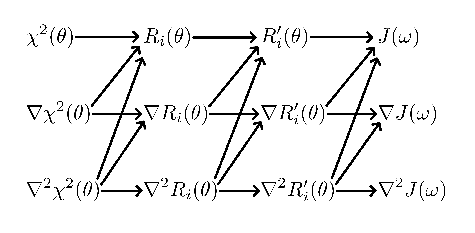
\includegraphics[width=0.8\textwidth]{images/dependencies/dependencies.eps}}
\caption{Dependencies between the $\chi^2$, transformed relaxation, relaxation, and spectral density equations, gradients, and Hessians.}\label{fig: dependencies}
\end{figure}



% Fully anisotropic rotational diffusion tensor.
%%%%%%%%%%%%%%%%%%%%%%%%%%%%%%%%%%%%%%%%%%%%%%%%

\newpage
\section{Fully anisotropic rotational diffusion tensor}

The fully anisotropic diffusion tensor can be specified in innumerable ways.  The shape of the tensor can be parameterised by the 


The weight equations containing directional cosines are preferential to the equations composed spherical coordinates.  This is because the partial and second partial derivatives of directional cosine dot products are much simpler than those of the spherical coordinate dot and cross products.  The three directional cosines of the fully anisotropic diffusion tensor are defined as

\begin{eqnarray}
    \delta_\alpha & = & \widehat{XH} . \widehat{D_x},   \label{eq: dir cos: da} \\
    \delta_\beta  & = & \widehat{XH} . \widehat{D_y},   \label{eq: dir cos: db} \\
    \delta_\gamma & = & \widehat{XH} . \widehat{D_z},   \label{eq: dir cos: dg} \\
\end{eqnarray}

\noindent where the set of Euler angles are

\begin{equation}
    \psi \ = \ \{\alpha, \beta, \gamma\}.   \label{eq: dir cos: euler}
\end{equation}


% Anisotropic weight derivatives (directional cosines).
%~~~~~~~~~~~~~~~~~~~~~~~~~~~~~~~~~~~~~~~~~~~~~~~~~~~~~~

\subsection{Anisotropic weight derivatives (directional cosines)}

\subsubsection{Equations}



